\chapter{Analisi di Downs}
\nocite{Enlow1986,Vorhies1951,Downs1956}

L'analisi di Downs si può definire un'analisi ``\textit{profilo-orientata}''. Il piano di riferimento è quello di Francoforte, e la valutazione verticale è fatta unicamente tramite il piano mandibolare e l'asse Y. Quest'analisi non presenta punti cefalometrici propri, ma si basa su misure utilizzate in numerose altre analisi.

{\Huge FIXME!}

Spesso quest'analisi viene accompagnata da una \textit{tabella di Voorhies e Adams}, che fornisce un quadro grafico delle dieci misurazioni dell'analisi.

In quest'analisi distinguiamo misurazioni ossee da misurazioni dentali (graficamente separate nel poligono di Voorhies e Adams).

\section{Misurazioni ossee}
\begin{table}[h]
%\footnotesize
\caption{Misurazioni ossee nell'analisi di Downs (valori in °)}
\begin{tabularx}{\textwidth}{>{\bfseries}lXcc}
\toprule
 & Punti di riferimento & Val. medio & Range normalità \\
\cmidrule(r){2-4}
Angolo facciale & \piano{Na}{Pog} -- \textit{FH} & 87.8 $\pm$ 3.6 & 82 -- 95 \\
Convessità facciale & \piano{Na}{A} -- \piano{A}{Pog} & 0 & -8.5 -- 10 \\
Piano \piano{A}{B} & \piano{A}{B} -- \piano{Na}{Pog} & -4.6 & -9 -- 0 \\
Piano mandibolare & \textit{MP} -- \textit{FH} & 21.9 & 17 -- 28 \\
Asse Y & \piano{S}{Gn} -- \textit{FH} & 59.4 & 53 -- 66 \\
\bottomrule
\end{tabularx}
\end{table}

\begin{figure}[h!]
\centering
\begin{minipage}{.44\textwidth}
 \centering
 \fbox{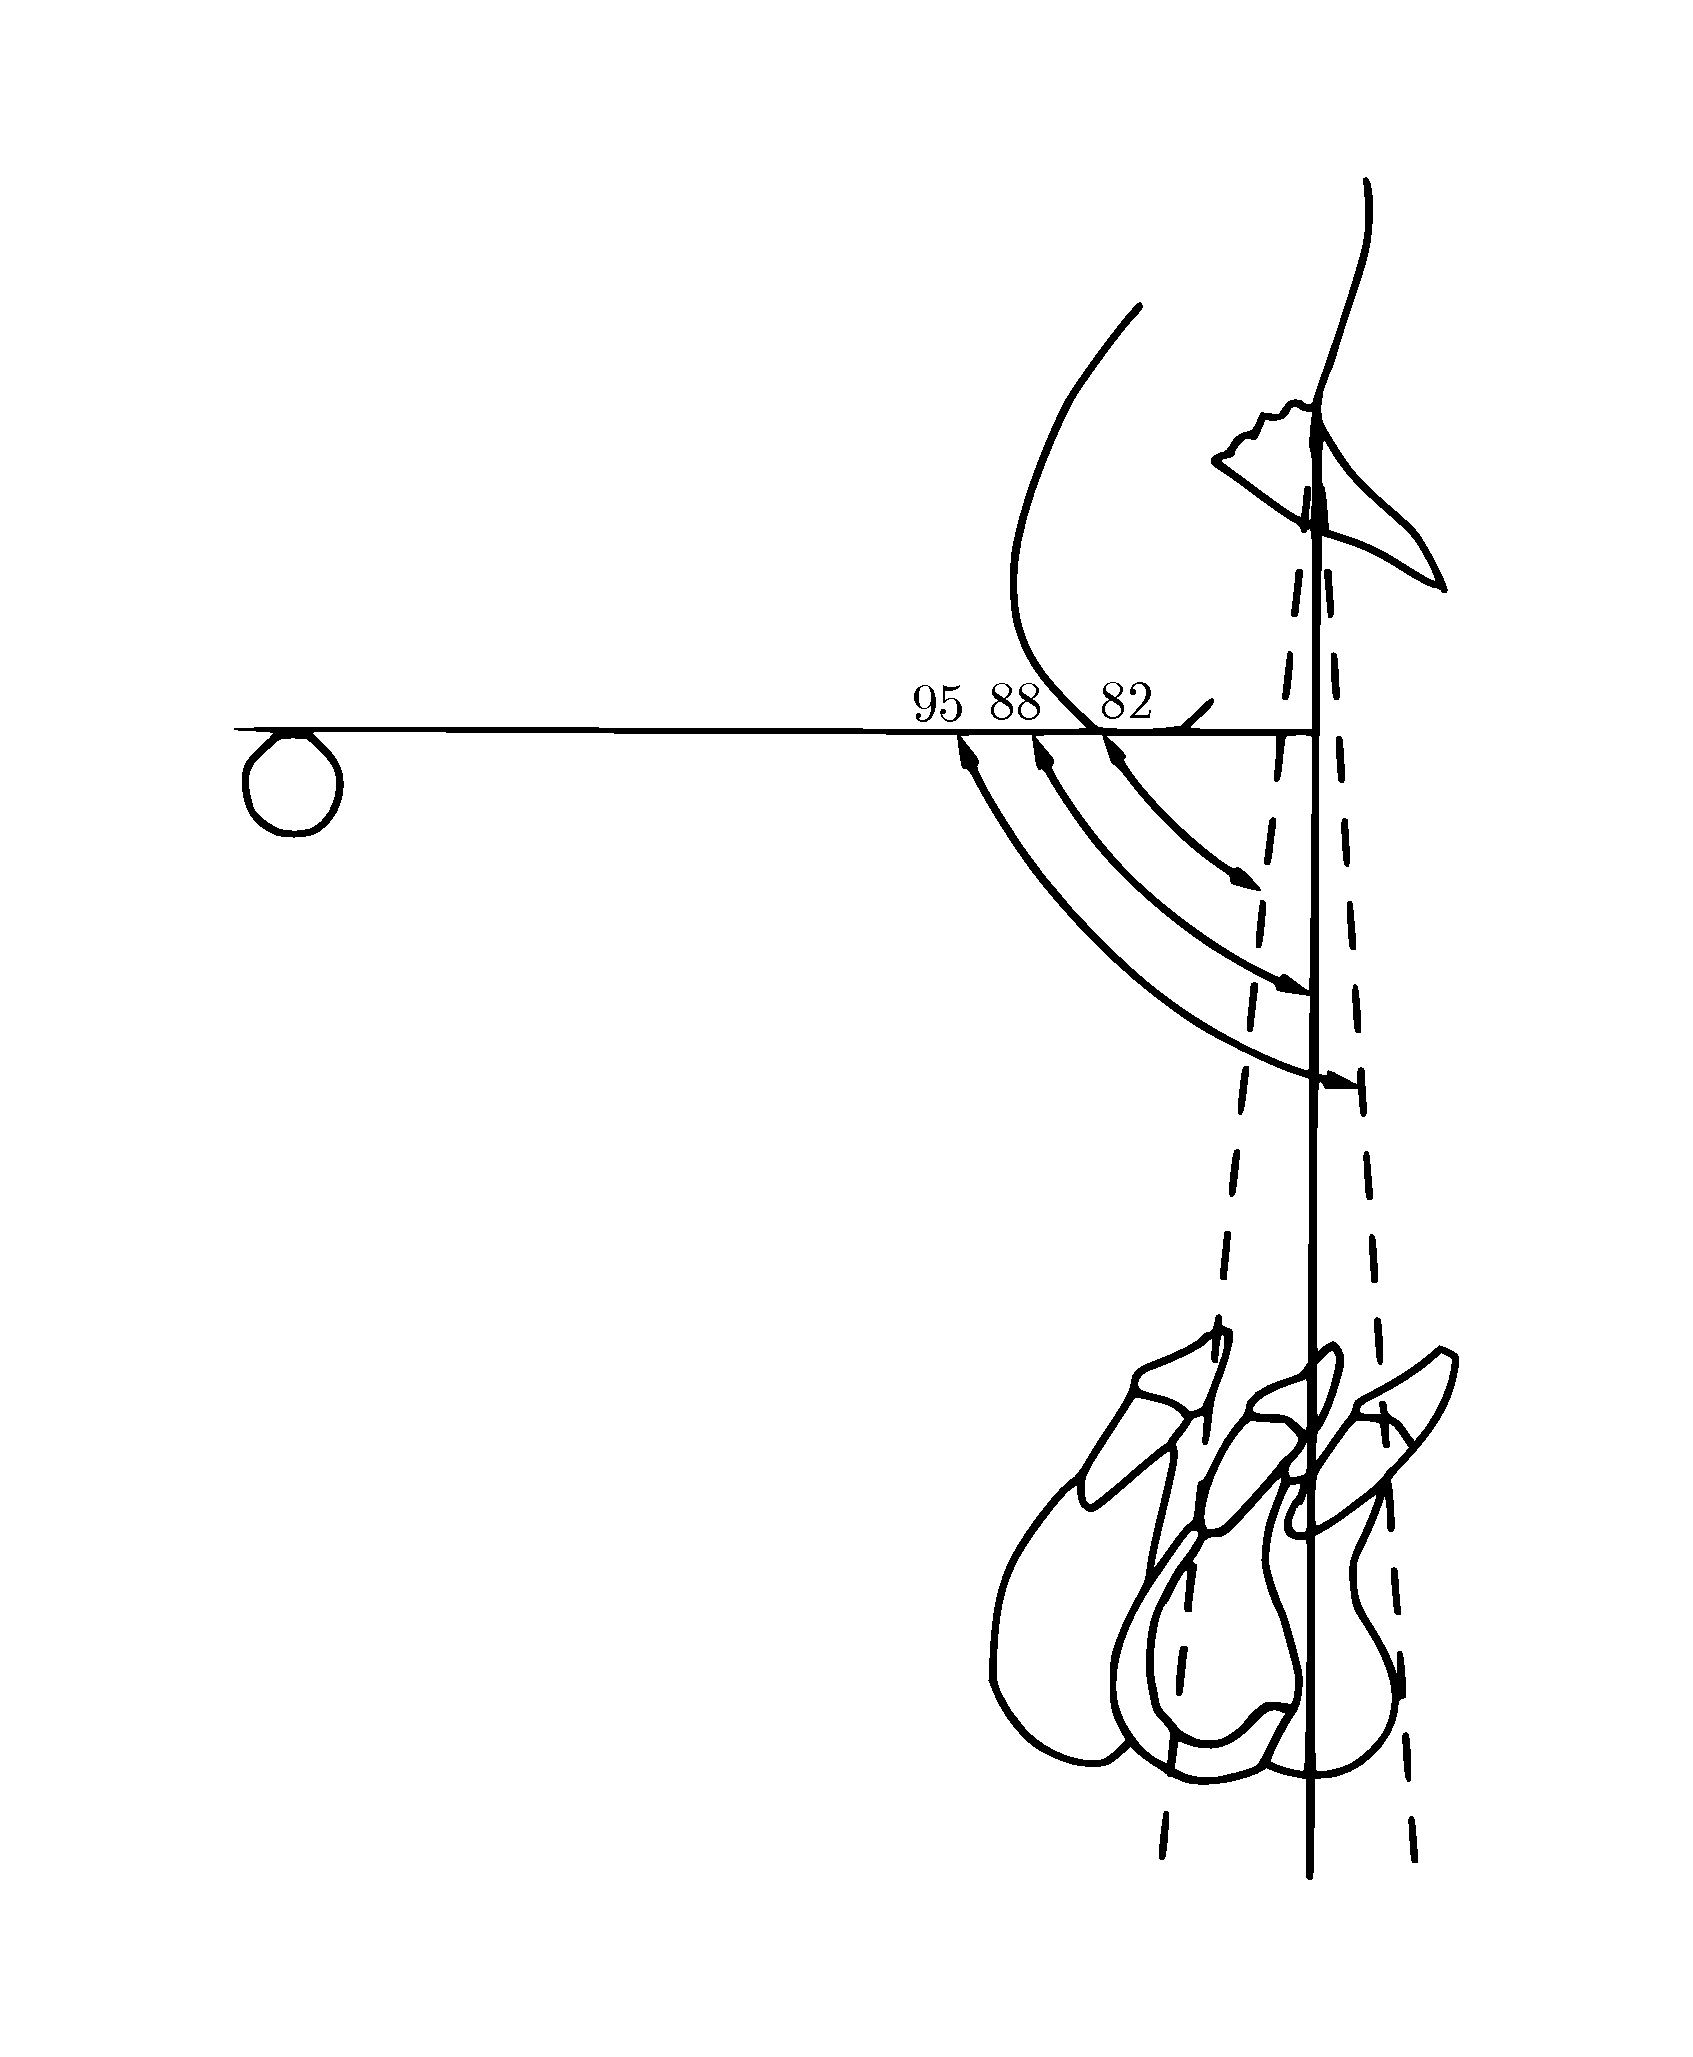
\includegraphics[width=.95\textwidth]{./images/downs_facciale.pdf}}
 \caption{Angolo facciale di Downs.}
 \label{fig:downs_facciale}
\end{minipage}\quad\quad
\begin{minipage}{.44\textwidth}
 \centering
 \fbox{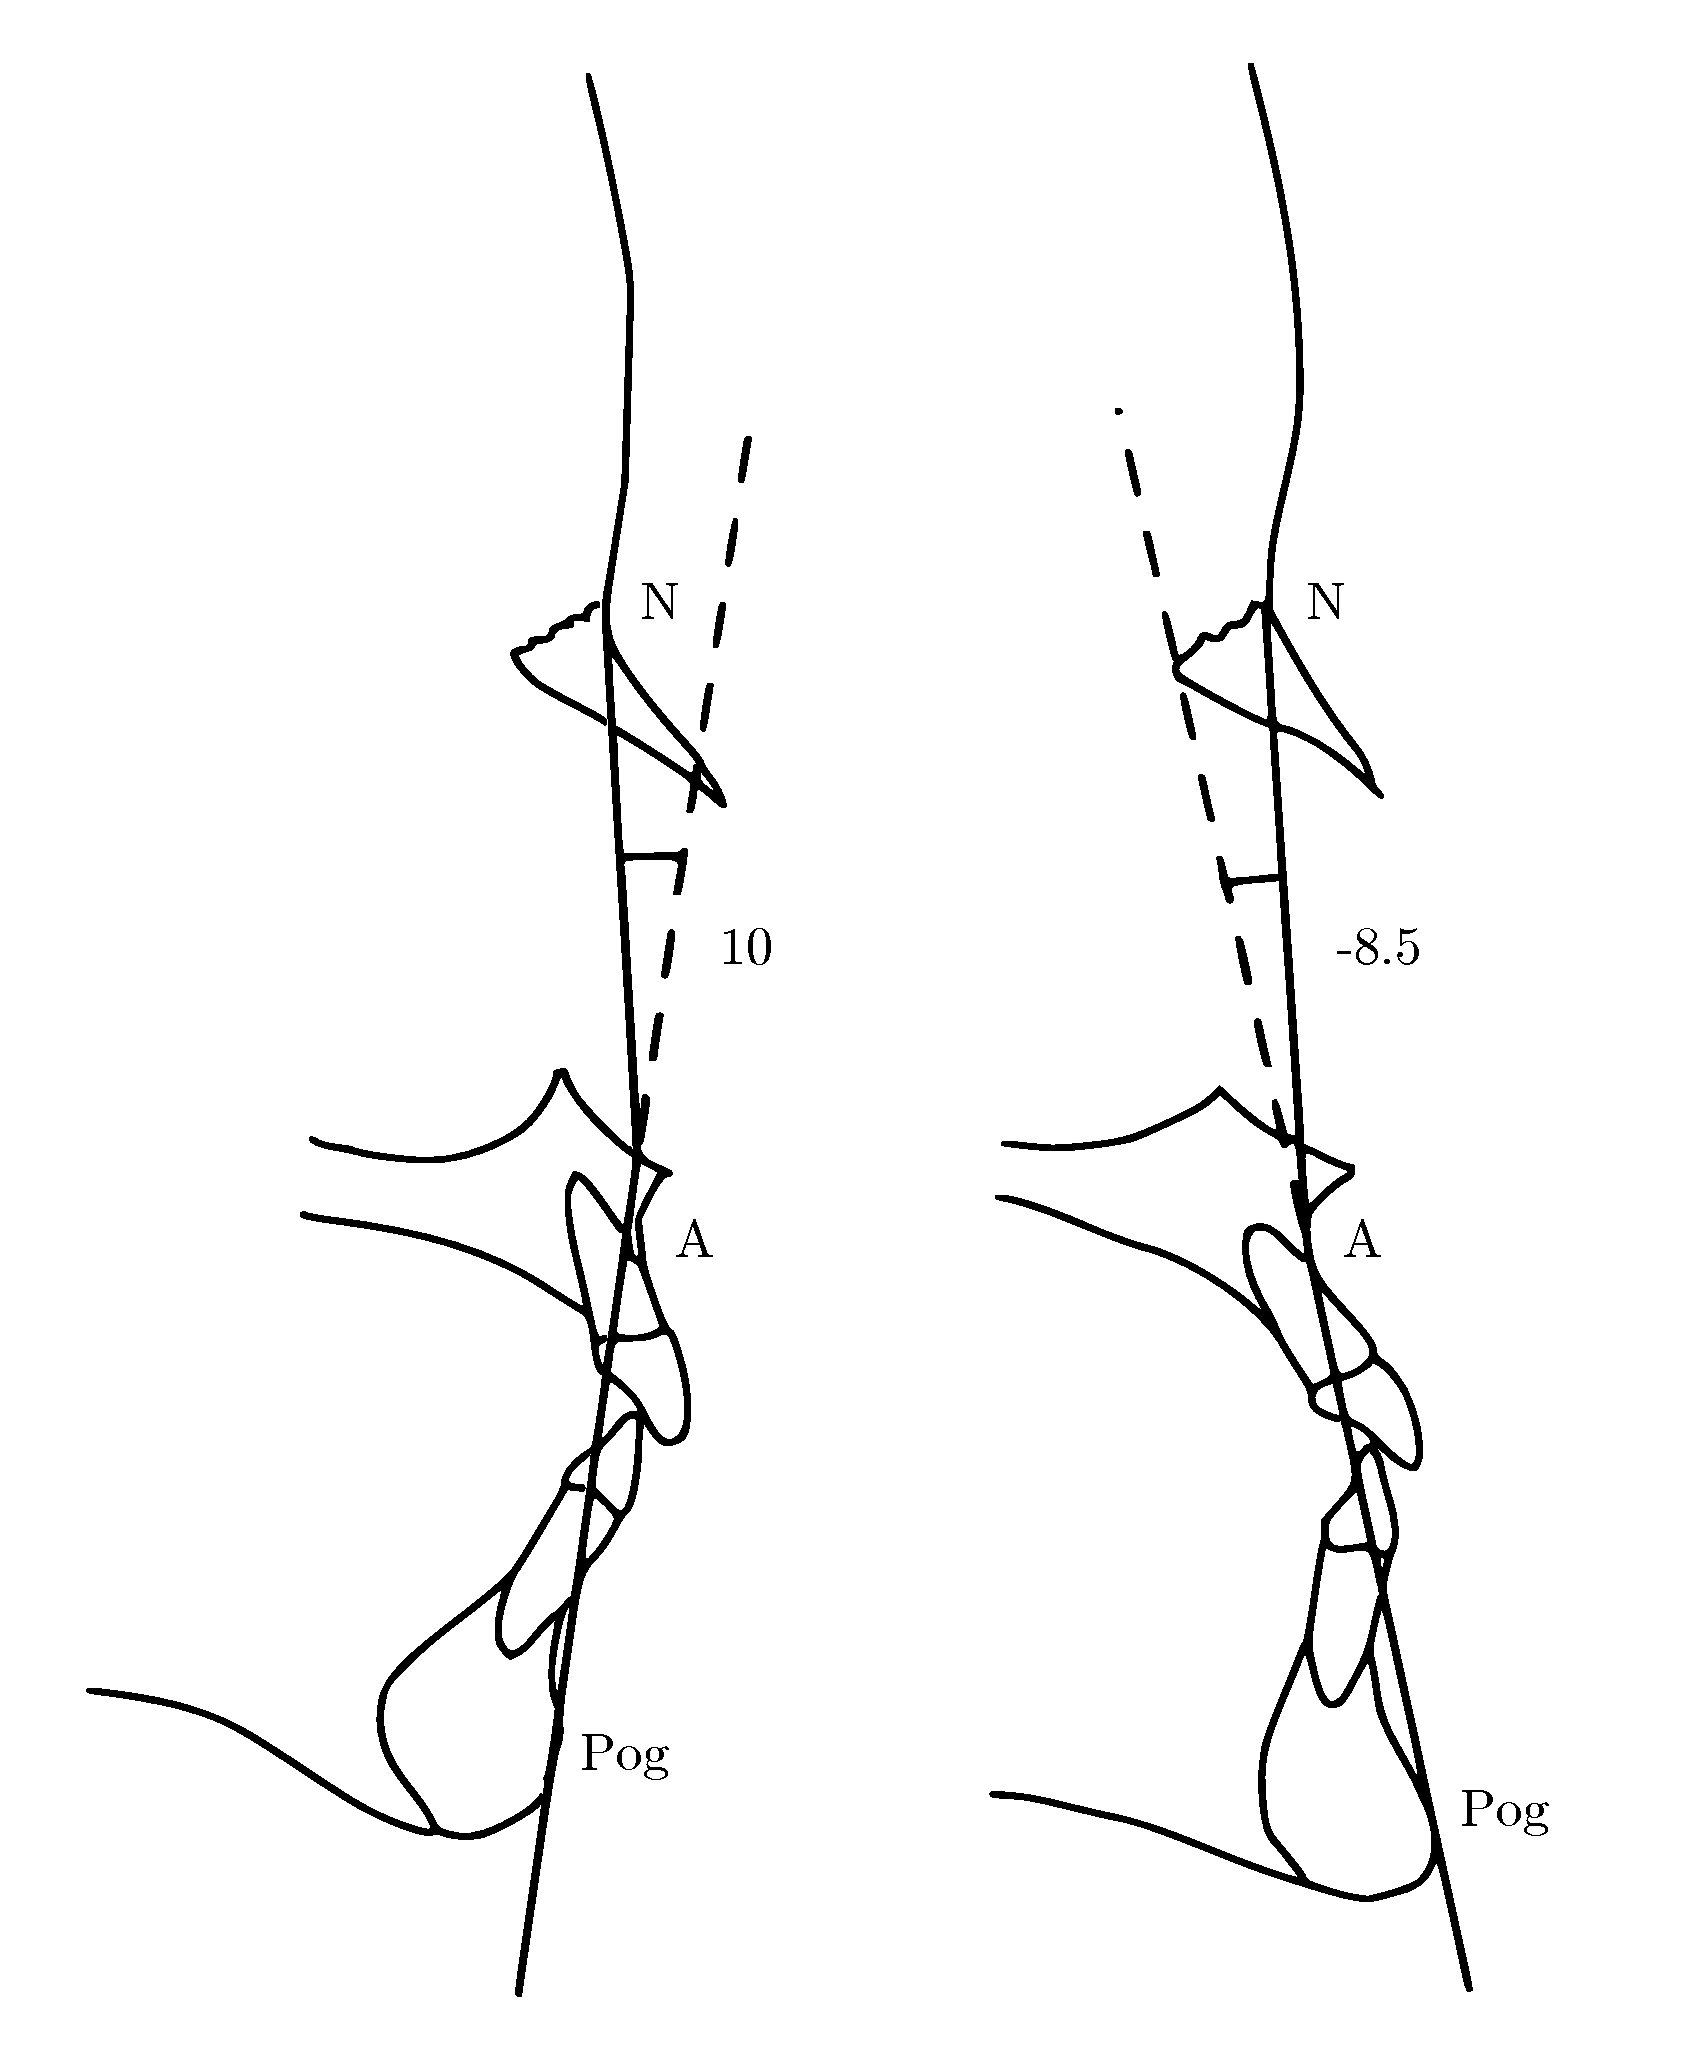
\includegraphics[width=.95\textwidth]{./images/downs_convessita.pdf}}
 \caption{Convessità facciale di Downs.}
 \label{fig:downs_convessita}
\end{minipage}
\end{figure}

\paragraph{Angolo facciale} (fig.~\ref{fig:downs_facciale}) usato per misurare il grado di retrusione o protrusione della mandibola. È l'angolo interno inferiore tra la linea facciale \piano{Na}{Pog} e il piano di Francoforte \textit{FH}. Ha un valore medio di 87.8 $\pm$ 3.6, con un range di normalità tra 82 e 95. Un mento prominente aumenta quest'angolo, un valore inferiore invece suggerisce una posizione retrusa del mento.

\paragraph{Convessità facciale} (fig.~\ref{fig:downs_convessita}) è un angolo formato dall'intersezione tra la linea \piano{Na}{A} e la linea \piano{A}{Pog}. Esso misura la relazione tra l'arco basale mascellare al suo limite anteriore (punto \punto{A}) e il profilo facciale totale (\piano{Na}{Pog}). Se la linea \piano{A}{Pog} tende in alto verso l'esterno, l'angolo è positivo. Un angolo positivo suggerisce una prominenza della base alveolare superiore rispetto alla mandibola. Un angolo negativo invece è associato ad un profilo prognatico. Il valore medio è di 0°, con un range di normalità tra -8.5° e 10°.

\paragraph{Piano \piano{A}{B}} (fig.~\vref{fig:downs_piano_ab}) forma un angolo con la linea \piano{Na}{Pog}, che indica la relazione tra i limiti anteriori dei processi alveolari e la linea facciale. Rappresenta una stima della difficoltà dell'ottenimento di una corretta inclinazione assiale e relazione tra gli incisivi dopo una terapia ortodontica. Poiché il punto \punto{B} è posizionato dietro il punto \punto{A}, quest'angolo è solitamente negativo, tranne che nelle Classi III o nelle Classi I con protrusione mandibolare. Un valore largamente negativo suggerisce una malocclusione di Classe II. Ha un valore medio di -4.6°, con un range di normalità tra -9° e 0°.

\begin{figure}[h!]
\centering
\begin{minipage}{.44\textwidth}
 \centering
 \fbox{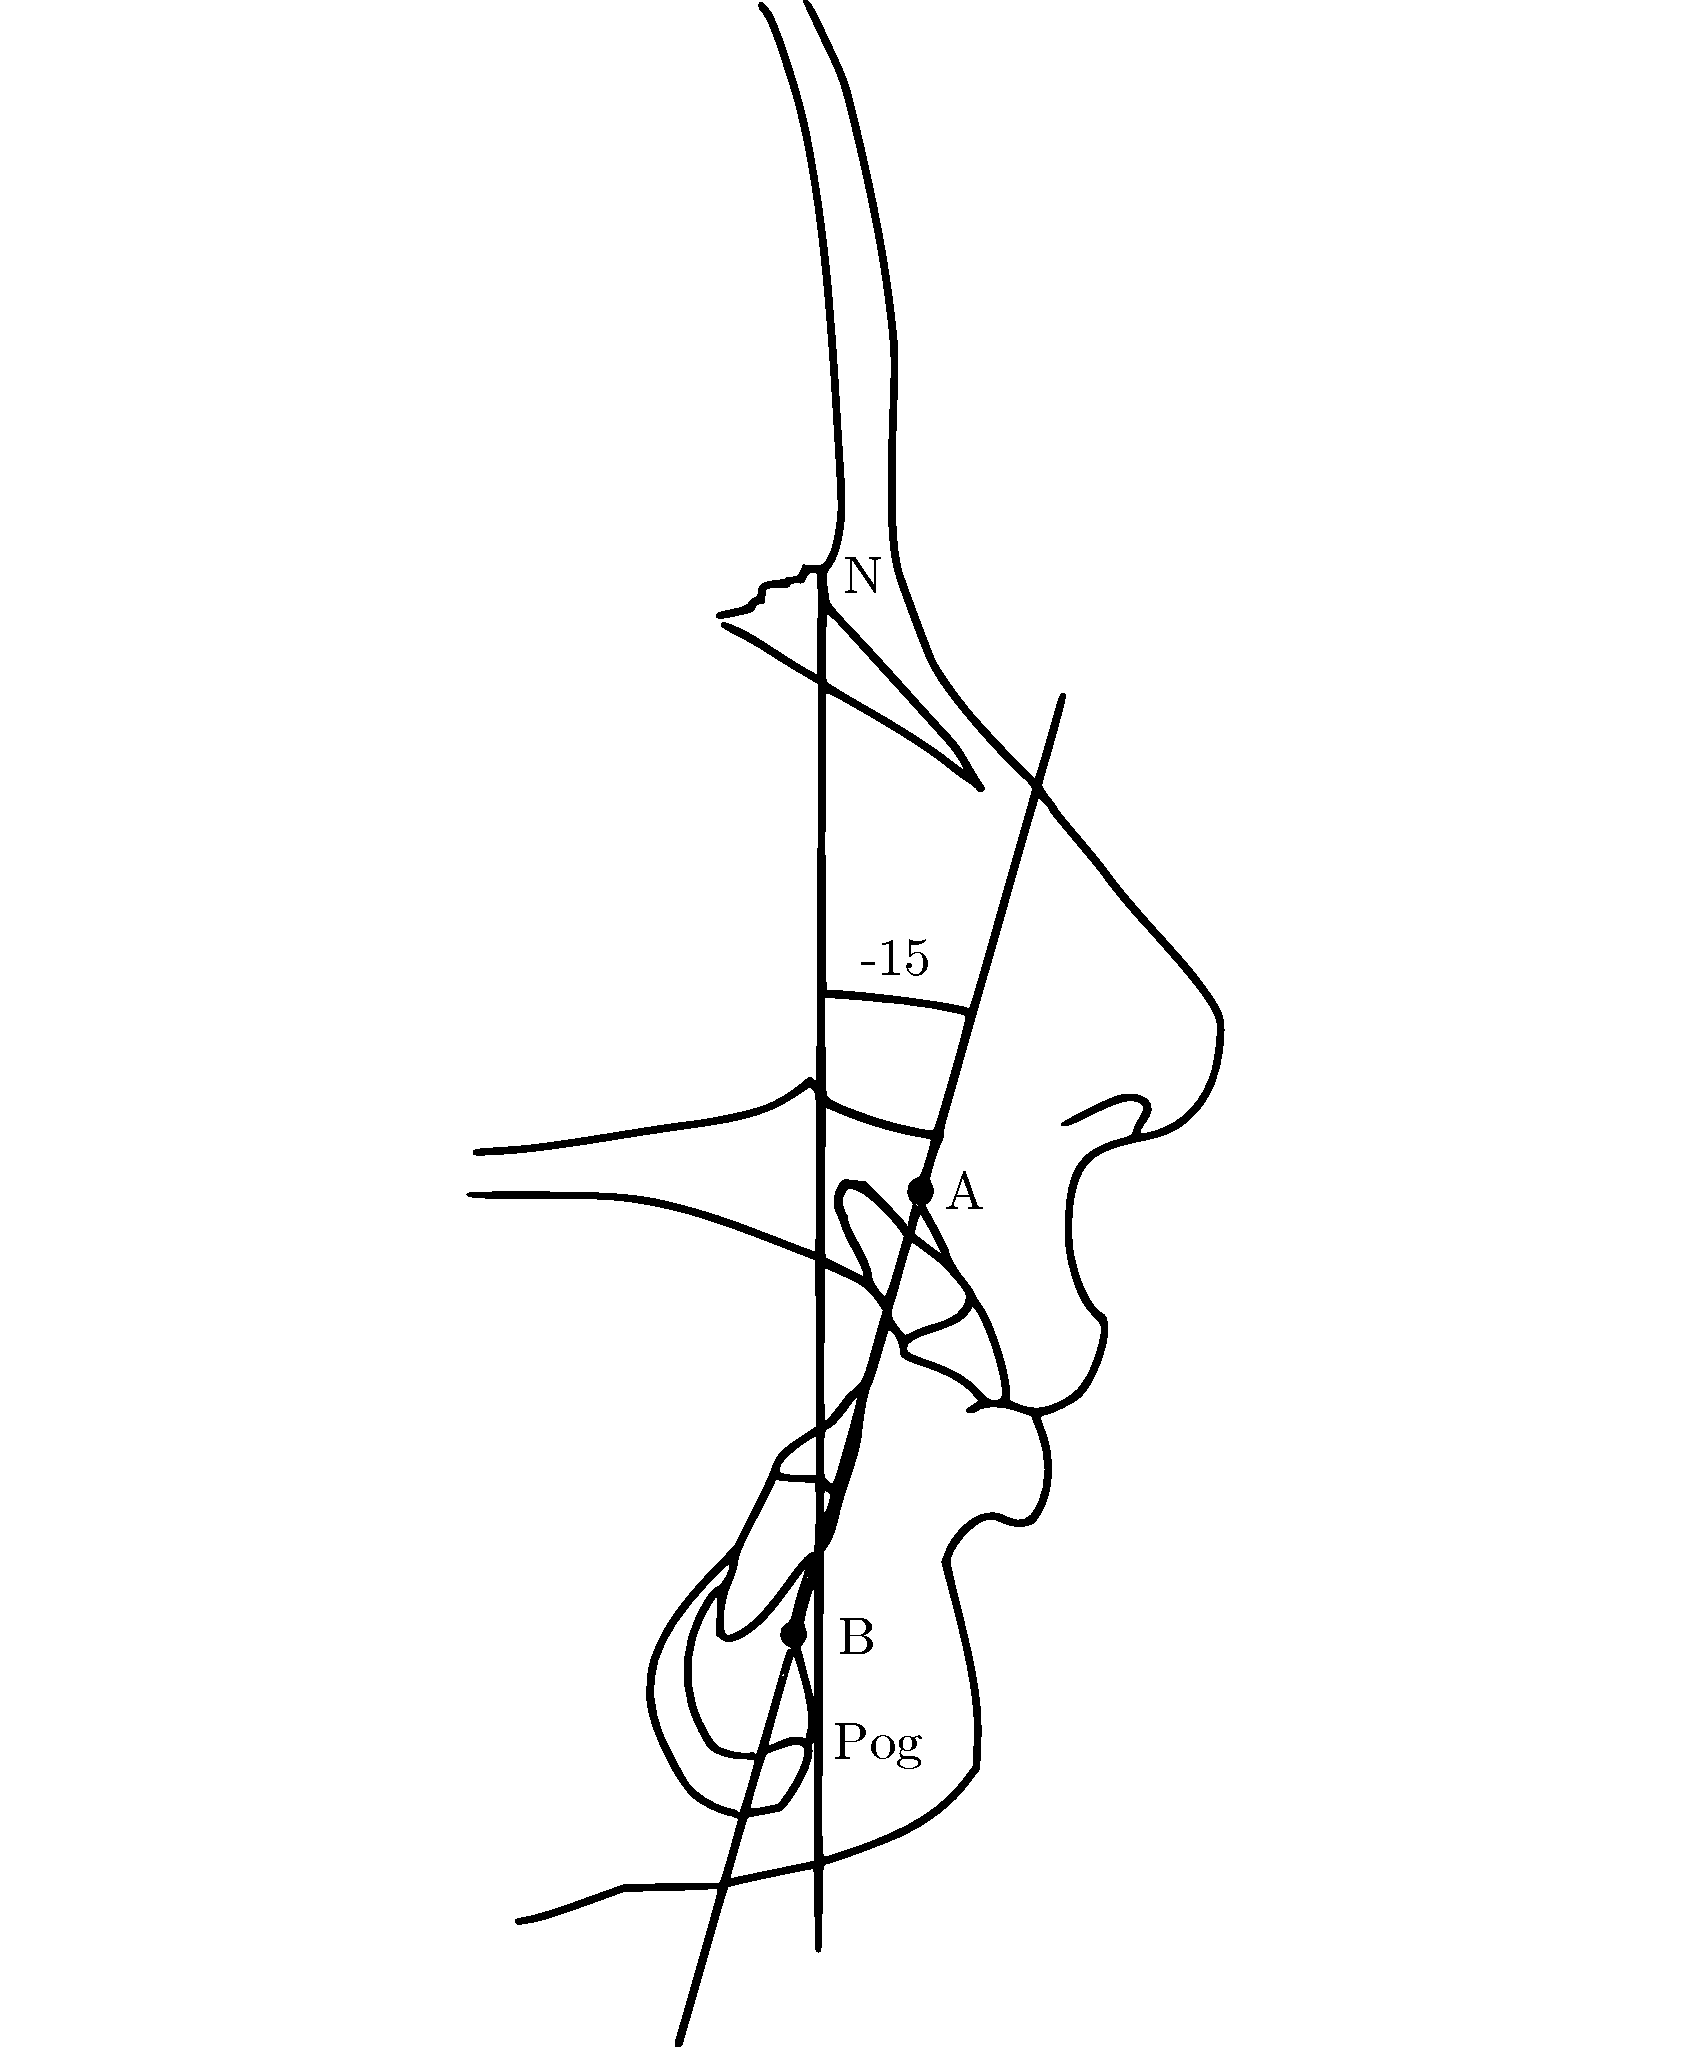
\includegraphics[width=.95\textwidth]{./images/downs_piano_ab.pdf}}
 \caption{Piano \piano{A}{B} di Downs.}
 \label{fig:downs_piano_ab}
\end{minipage}\quad\quad
\begin{minipage}{.44\textwidth}
 \centering
 \fbox{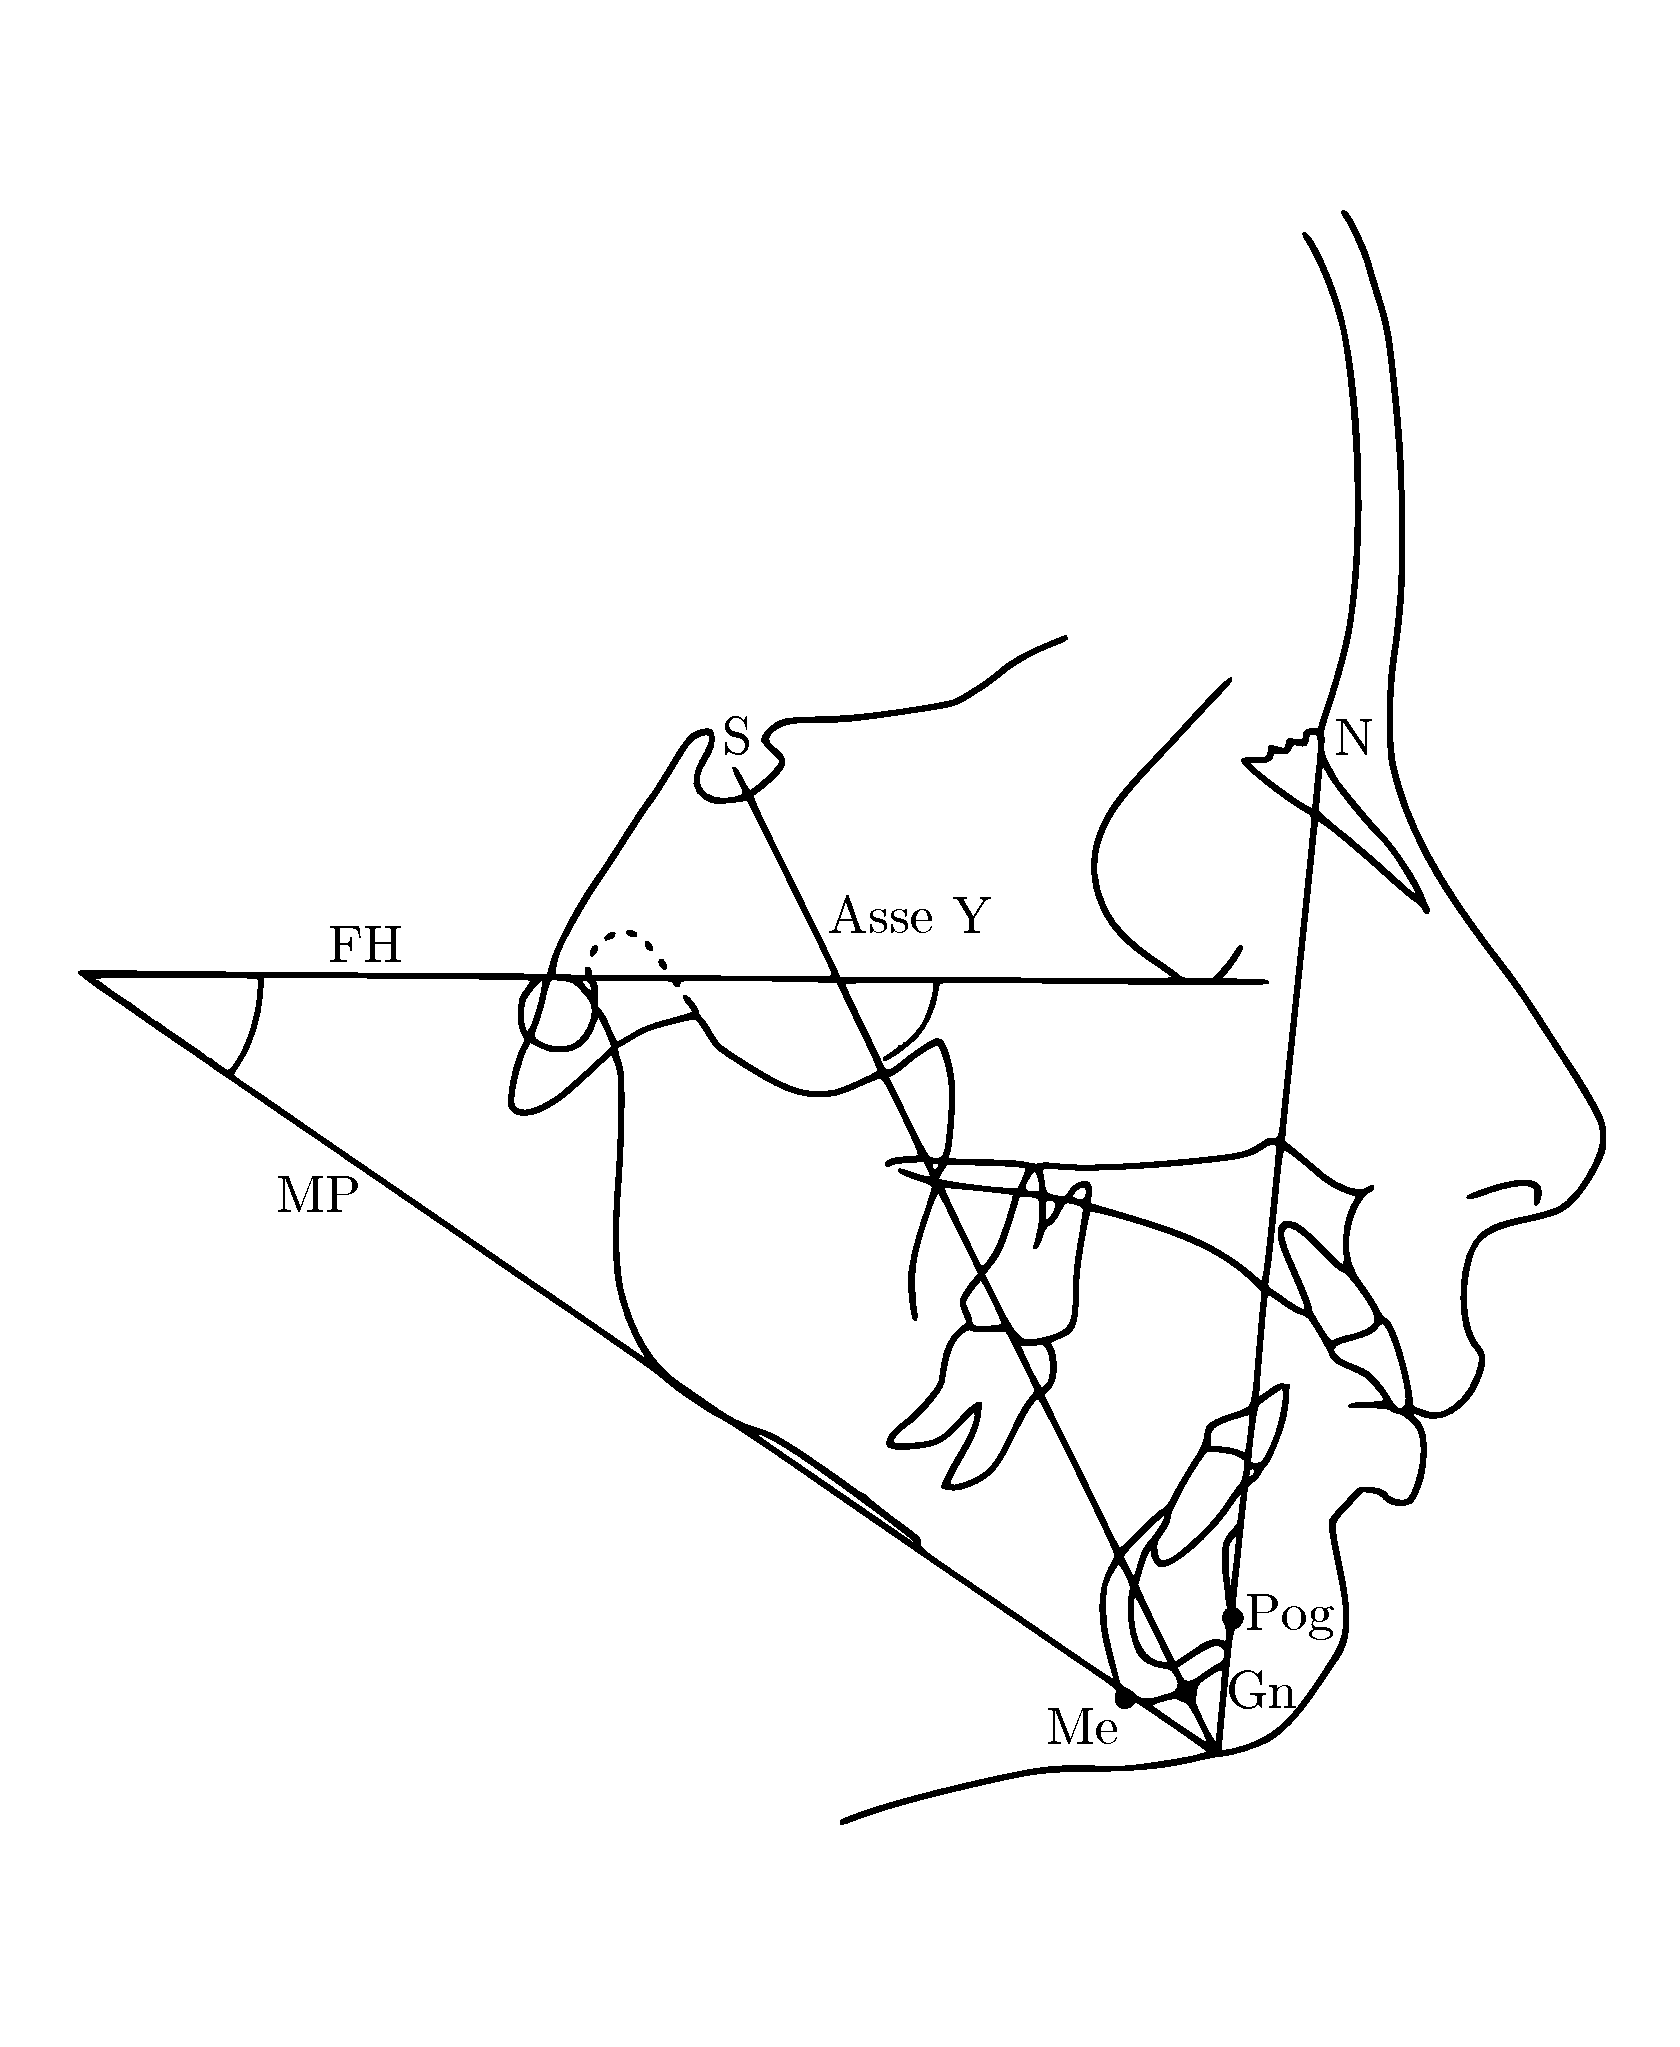
\includegraphics[width=.95\textwidth]{./images/downs_mandibolare_asse_y.pdf}}
 \caption{Piano mandibolare e Asse Y.}
 \label{fig:downs_mandibolare_asse_y}
\end{minipage}
\end{figure}

\paragraph{Piano mandibolare} (fig.~\vref{fig:downs_mandibolare_asse_y}) tangente all'angolo goniaco e al punto più inferiore della sinfisi mentoniera. L'angolo viene misurato dalla relazione tra il piano mandibolare e il piano di Francoforte. Si riscontrano valori elevati sia in soggetti retrusi e protrusi, e suggeriscono pattern facciali iperdivergenti, poco favorevoli al trattamento: essi risultano infatti complicati, con una prognosi incerta. Quest'angolo, però, non è sufficiente a indicare la natura della difficoltà che si potrà riscontrare durante il trattamento. Ha un valore medio di 21.9°, con un range di normalità tra 17° e 28°.

\paragraph{Asse Y} (fig.~\ref{fig:downs_mandibolare_asse_y}) rappresenta l'asse di crescita facciale, e indica la posizione in basso, o indietro, o in avanti del mento in relazione alla faccia superiore. Il relativo angolo è misurato all'intersezione della linea \piano{S}{Gn} e il piano di Francoforte. Quest'angolo è maggiore nelle Classi II rispetto alle Classi tendente-III. Un decremento di questo valore in radiografie seriali può essere interpretato come una crescita orizzontale prevalente su quella verticale. Ha un valore medio di 59.4°, con un range di normalità tra 53° e 66°.

\section{Misurazioni dentali}
\begin{table}[h]
%\footnotesize
\begin{tabularx}{\textwidth}{>{\bfseries}lXcc}
\toprule
 & Punti di riferimento & Val. medio & Range normalità \\
\cmidrule(r){2-4}
Piano occlusale (°) & \textit{PO} -- \textit{FH} & 9.3 & 1.5 -- 14 \\
Angolo interincisale (°) & assi inc. centrali & 135.4 & 130 -- 150.5 \\
Piano inc.-occlusale (°) & \textit{PO} -- asse inc. inf. & 14.5 $\pm$ 3.5 & 3.5 -- 20 \\
Piano inc.-mandibolare (°) & \textit{MP} -- asse inc. inf. & 1.4 & -8.5 -- 7 \\
Protr. inc. sup. (mm) & marg. inc. -- \piano{A}{Pog} & 2.7 & -1 -- 5 \\
\bottomrule
\end{tabularx}
\end{table}

\begin{figure}[h!]
 \centering
 \fbox{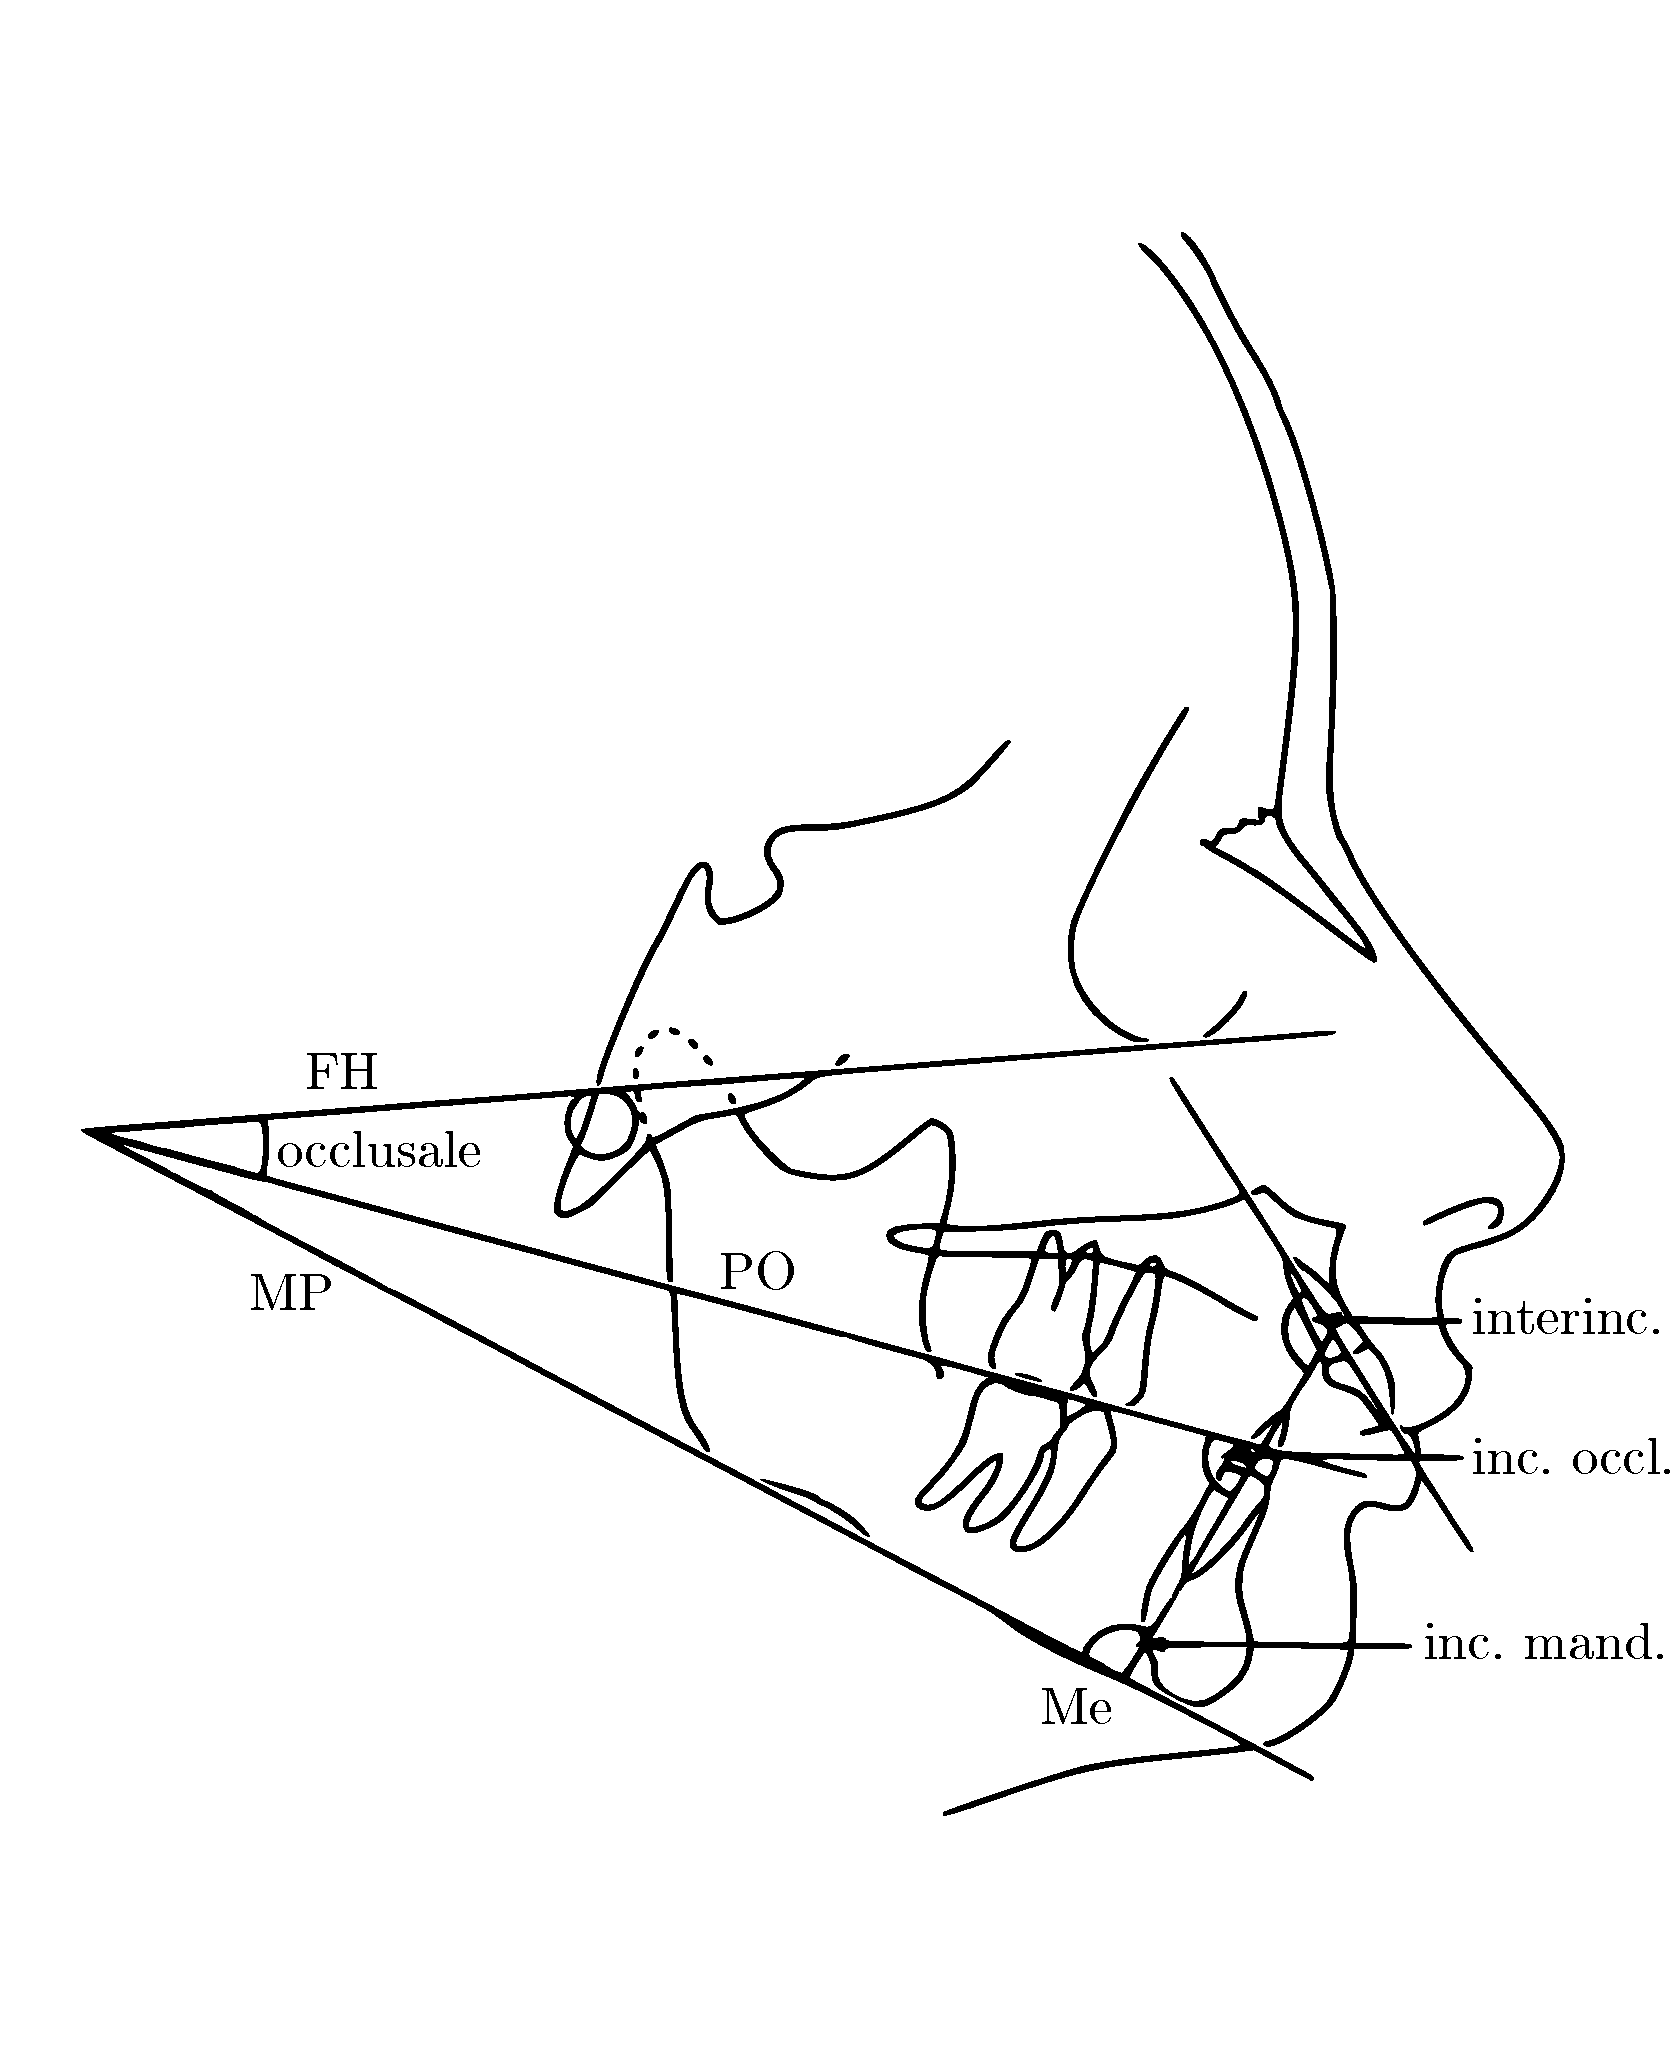
\includegraphics[width=.5\textwidth]{./images/downs_angoli_incisali_occlusale.pdf}}
 % downs_angoli_incisali_occlusale.pdf: 806x982 pixel, 72dpi, 28.43x34.64 cm, bb=0 0 806 982
 \caption{Angoli del piano occlusale, interincisale, incisivo-occlusale e incisivo-mandibolare.}
 \label{fig:downs_angoli_incisali_occlusale}
\end{figure}

\paragraph{Piano occlusale} (fig.~\ref{fig:downs_angoli_incisali_occlusale}) originariamente definito da Downs come la linea secante le cuspidi dei primi molari e l'overbite incisale. Nei casi di grossolana malposizione degli incisivi, Downs suggeriva di disegnare la linea secante le cuspidi dei primi molari e dei primi premolari. Il rispettivo angolo viene misurato tra il piano occlusale e il piano di Francoforte. Quando la parte anteriore del piano è posizionata più in basso rispetto alla parte posteriore, l'angolo è positivo. Angoli grandemente positivi si riscontrano in profili di Classe II, mentre risulta ridotto in casi di lunghi rami mandibolari. Ha un valore medio di 9.3°, con un range di normalità tra 1.5° e 14°.

\paragraph{Angolo interincisale} (fig.~\ref{fig:downs_angoli_incisali_occlusale}) viene stabilito tra gli assi maggiori degli incisivi centrali superiori ed inferiori. Ha un valore medio di 135.4°, con un range di normalità tra 130° e 150.5°.

\paragraph{Angolo piano incisivo-occlusale} (fig.~\ref{fig:downs_angoli_incisali_occlusale}) correla gli incisivi inferiori alla loro superficie lavorante. Viene misurato tra l'asse dell'incisivo inferiore e il piano occlusale, ha un valore medio di 14.5° $\pm$ 3.5°, con un range di normalità tra 3.5° e 20°.

\paragraph{Angolo piano incisivo-mandibolare} (fig.~\ref{fig:downs_angoli_incisali_occlusale}) è formato dall'intersezione del piano mandibolare con l'asse dell'incisivo inferiore. Quest'angolo è positivo quando gli incisivi sono inclinati in avanti rispetto al processo alveolare. Ha un valore medio di 1.4°, on un range di normalità tra -8.5° e 7°.

\begin{wrapfigure}{R}{.4\textwidth}
 \centering
 \fbox{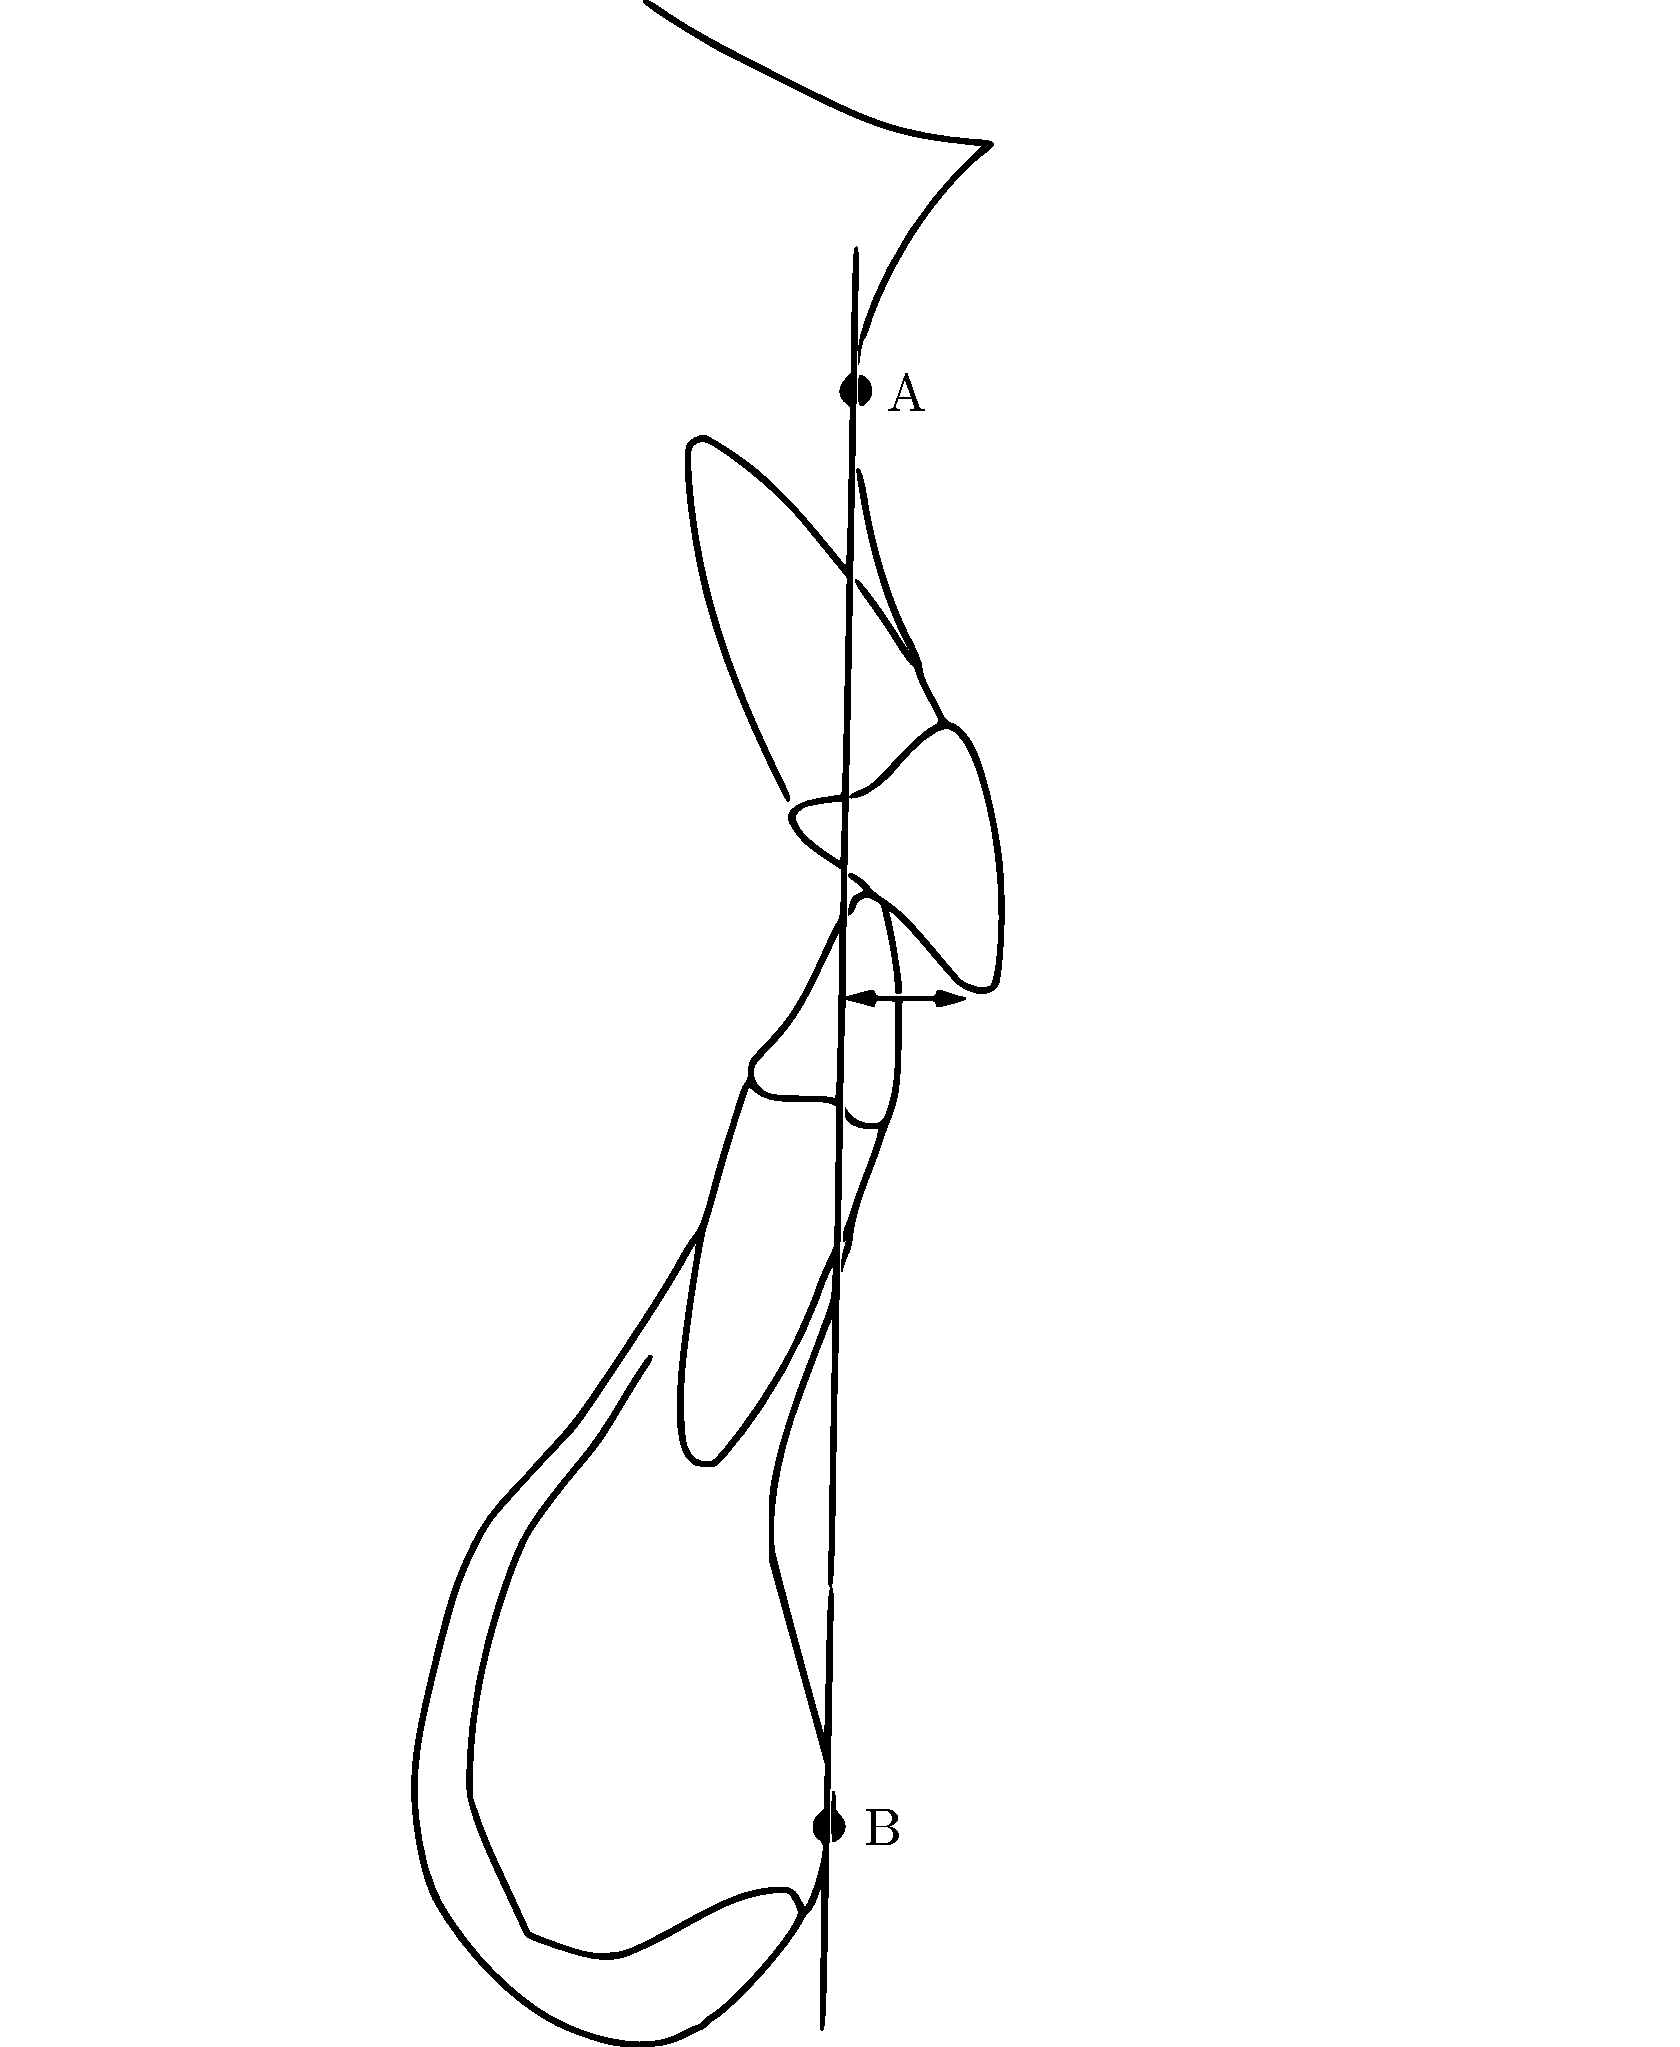
\includegraphics[width=.4\textwidth]{./images/downs_protrusione.pdf}}
 % downs_protrusione.pdf: 806x982 pixel, 72dpi, 28.43x34.64 cm, bb=0 0 806 982
 \caption{Protrusione incisivo superiore}
 \label{fig:downs_protrusione}
\end{wrapfigure}

\paragraph{Protrusione incisivi mascellari} (fig.~\ref{fig:downs_protrusione}) viene misurata in millimetri, come la distanza tra il margine incisale superiore e la linea \piano{A}{Pog}. La distanza è positiva se il margine incisale cade al davanti di tale linea, e indica la quantità di protrusione mascellare. Il valore medio è di 2.7mm, con un range di normalità tra -1mm e 5mm.
